\documentclass[twoside,UTF8]{EPURapport}
%\usepackage{listings}

%\renewcommand{\lstlistlistingname}{Liste des codes}
%\renewcommand{\lstlistingname}{Code}

%\addextratables{%
%	\lstlistoflistings
%}

%\swapAuthorsAndSupervisors
\usepackage{float}


\thedocument{Rapport de projet}{Développement d'un site de vente et de gestion pour la Kfet de Polytech}{Site web Kfet}

\grade{Département Informatique\\ 5\ieme{} année\\ 2011 - 2012}

\authors{%
	\category{Étudiants}{%
		\name{Loïc CARNEY} \mail{loic.carney@etu.univ-tours.fr}
		\name{Sébastien LACROIX} \mail{sebastien.lacroix@etu.univ-tours.fr}
	}
	\details{DI5 2008 - 2009}
}

\supervisors{%
	\category{Encadrants}{%
		\name{Alexandre LISSY} \mail{alexandre.lissy@univ-tours.fr}
	}
	\details{Université François-Rabelais, Tours}
}

\abstracts{Description en français}
{Mots clés français}
{Description en anglais}
{Mots clés en anglais}

\begin{document}
\renewcommand{\labelitemi}{\textbullet}

\chapter{Introduction}%{{{

    \paragraph{}Dans le cadre de notre dernière année d'étude à Polytech'Tours, nous devions réaliser un projet lié aux technologies web. Nous avons décider de proposer notre propre sujet. L'un de nous ayant été trésorier à la Kfet du département Informatique de l'école, nous étions au courant que toute la gestion de la Kfet se fait sur papier et manuellement. Aucune gestion automatique n'est en place et aucune gestion des stocks n'est effectuée pour le moment. Nous avons donc proposer comme sujet : la réalisation d'un site web permettant de répondre à tous les besoins de gestion de la Kfet: en commençant par la vente jusqu'à la gestion des stocks et en passant par la gestion des dettes.

    \paragraph{}Pour réaliser le projet web, nous avons décidé d'utiliser une technologie web que nous ne connaissions pas : le  framework web Django qui est basé sur le langage interprêté Python. Le but de Django est de donner au développeur web des outils simples et rapides, en effet son slogan est "Le framework web pour les perfectionnistes sous pression".

    \paragraph{}La Kfet de Polytech est ouverte à toutes les pauses. Lors des pauses d'inter-cours elle vend des en-cas, confiseries et des boissons chaudes,et lors de la pause de midi elle sert des plats chauds. Les stocks sont donc assez conséquents et varient fortement, la problématique de la gestion des stocks est un des éléments qui nous a incité à réaliser ce projet.

    \paragraph{}Nous allons donc vous présenter tout d'abord le projet au travers du cahier des charges puis nous détaillerons le fonctionnement de chaque module mis en place.
%}}}

%%%%%%%%%%%%%%%%%%%%%%%%%%%%%%%%%%%%%%%%%%%%%%%%%%%%%%%%%%%%%%%%%%%%%%%%%%%%%%%%%%%%%%%%%%%%%%%%%%%%ù
%%%%%%%%%%%%%%%%%%%%%%%%%%%%%%%%%%%%%%%%%%%%%%%%%%%%%%%%%%%%%%%%%%%%%%%%%%%%%%%%%%%%%%%%%%%%%%%%%%%%ù
%%%%%%%%%%%%%%%%%%%%%%%%%%%%%%%%%%%%%%%%%%%%%%%%%%%%%%%%%%%%%%%%%%%%%%%%%%%%%%%%%%%%%%%%%%%%%%%%%%%%ù
\chapter{Cahier des charges}%{{{
% TODO Seb

    \paragraph{}Nous allons dans cette partie définir les fonctionnalités attendues par la Kfet afin de simplifier la vie de ses membres. Nous allons pour cela décomposer les fonctionnalités par rôles de l'association. 
    \paragraph{}Nous allons donc dans un premier temps définir les fonctionnalités de gestion d'association, puis les fonctionnalités d'un kftier vendeur, enfin nous définirons les fonctionnalités proposés à un étudiant non membre de l'association.

    \section{Fonctionnalités de gestion}

        \paragraph{}Le but premier de ce projet était de remettre en place une réelle gestion au sein de la Kfet. Nous voulions ainsi permettre de suivre en détails les stocks, les ventes de la journée ou du mois, le chiffre d'affaire ...

        \subsection{Gestion des stocks}

            \paragraph{}Le manque de gestion administrative de la Kfet entraine une faiblesse majeure : presque aucune gestion des stocks n'est assurée. Cette faiblesse se ressent le plus lors du manque de pizza le midi et le mécontentement des clients qui en découle.
            \paragraph{}Nous nous proposons donc de mettre en place une gestion des stocks complète apportant les fonctionnalités suivantes :\\
            \begin{itemize}
                \item Ajout de fournisseur : Pouvoir avoir plusieurs fournisseur différents, notamment afin de pouvoir différencier les commandes ;\\
                \item Commande de produit : Pouvoir avoir une trace de la commande effectué auprès du fournisseur et ne la valider qu'une fois arrivée. Nous voulons ainsi différencier les produits en stocks, des commandes ;\\
                \item Notification de fin de stock : Recevoir une notification par mail lorsqu'un stock atteint le seuil limite afin de pouvoir réapprovisionner avant la rupture.\\
            \end{itemize}

        \subsection{Gestion des finances}

            \paragraph{}Nous voulions apporter à la Kfet des outils de gestion permettant d'avoir des informations sur les ventes, le chiffre d'affaire ... Ces outils pourrons par exemple permettre de mettre en avant des pertes trop importantes sur certains produits. Nous avons donc définis les fonctionnalités suivantes :\\

            \begin{itemize}
                \item Statistiques de ventes : afficher le chiffre d'affaire, les ventes réalisées sur une période définie ;\\
                \item Gestion des dettes : pouvoir gérer les dettes de tous les clients de façon informatique (enseignants et étudiants) et pouvoir les avertir lorsqu'un plafond est atteint.
            \end{itemize}

    \section{Fonctionnalités de vente}
        
        \paragraph{}Afin de simplifier la gestion de stock et le fonctionnement de la Kfet nous avons voulu proposer des fonctionnalités de ventes. 

        \paragraph{}La partie vente se décompose en deux types : les commandes de menus le midi, et les ventes individuelles.

        \subsection{Gestion des commandes}
            \paragraph{}Les fonctionnalités permettant de gérer les commandes vont permettre de supprimer tous le système complexe et non productif des papiers de commande. Nous proposons donc les fonctions suivantes :
        
            \begin{itemize}
                \item Gestion de commandes : validation, paiement, annulation ;\\                
                \item Historique permettant un calcul de chiffre d'affaire.
            \end{itemize}

        \subsection{Ventes}
            \paragraph{}Afin de pouvoir avoir une gestion des stocks complète il faut qu'une chaque vente soit enregistrée de manière informatique. Pour cela nous proposons de mettre en place une interface facilement adaptable à un appareil tactile permettant de vendre à l'unité ou en lot et permettant de mettre la vente en dette. Une gestion avancée de celles-ci pourra de plus être mise en place permettant d'annuler la vente en cas d'erreur par exemple.

    \section{Fonctionnalités utilisateur}

        \paragraph{}Nous avons voulu proposer des fonctionnalités simplifiant la gestion de la Kfet, mais nous voulons aussi proposer des fonctionnalités intéressantes aux clients.

        \paragraph{}Nous proposons pour cela de mettre en place un site de e-commerce permettant de réaliser n'importe quelle commande en avance. Cela évitera, par exemple, dans le cas de la vente de pizza la cohue au comptoir due au nombre limité de commande.

        \paragraph{}Un compte utilisateur permettra de plus de pouvoir consulter sa dette, voire de la régler par carte bleue ou paypal.
        %}}}

%%%%%%%%%%%%%%%%%%%%%%%%%%%%%%%%%%%%%%%%%%%%%%%%%%%%%%%%%%%%%%%%%%%%%%%%%%%%%%%%%%%%%%%%%%%%%%%%%%%%ù
%%%%%%%%%%%%%%%%%%%%%%%%%%%%%%%%%%%%%%%%%%%%%%%%%%%%%%%%%%%%%%%%%%%%%%%%%%%%%%%%%%%%%%%%%%%%%%%%%%%%ù
%%%%%%%%%%%%%%%%%%%%%%%%%%%%%%%%%%%%%%%%%%%%%%%%%%%%%%%%%%%%%%%%%%%%%%%%%%%%%%%%%%%%%%%%%%%%%%%%%%%%ù
\chapter{Le framework Django}

\section{Présentation}
Afin de réalisrer notre site web, nous avons choisi d'utiliser Django. Django est un framework web Python de haut niveau qui a comme slogan :\\
\begin{center}
    \begin{LARGE}
    The web framework for perfectionnists with deadlines
    \end{LARGE}
\end{center}

Cela signifie : "Le framework web pour les perfectionnistes sous pression". Ce qui nous correspond parfaitement.

\begin{figure}[H]
 \centering
 
\includegraphics[width=0.5\linewidth]{./logos/pony.jpg}
 \caption{Le logo représentatif de Django}
\end{figure}

Le framework Django est composé d'une multitude d'outils très puissant. De plus il est basé sur le modèle de framework MVT :
\begin{itemize}
    \item Modèle : C'est ici que nous définiront les objets que nous manipulons sur le site, en l'occurrence nos objets de base de données ;
    \item Vue : Permet de manipuler les objets de la base de données et les envoies aux pages HTML qui sont générées en fonction de la demande de l'utilisateur ;
    \item Template : Spécifie la structure de la page HTML. On y indique commet et où afficher les variables sur la page.
\end{itemize}

\paragraph{Pourquoi avoir choisir Django ?} Étant en école d'ingénieurs, il est très important d'avoir la volonté d'apprendre constamment de nouvelles technologies. Et cette année, nous avons entendu parlé du langage Python. Python est un langage très simple et très facile à apprendre.



\section{Outils très utiles}
Django possède toute une panoplie d'outils très utiles. Voici quelques uns des outils que nous avons utilisé :
\begin{itemize}
    \item Moteur de réécriture d'URL ;
    \item Moteur de template ;
    \item Serveur web de développement ;
    \item ORM compatible avec la base de données MySQL ;
    \item Moteur de formulaire ;
    \item Interface d'administration.
\end{itemize}

Dans cette section sera décrit brièvement chacun des outils afin de comprendre la facilité d'usage de Django. On peut retrouver facilement sur le site officiel de Django \url{https://www.djangoproject.com/} toute la documentation ainsi que des tutoriels permettant d'apprendre son fonctionnement.

    \subsection{Moteur de réécriture d'URL}
Afin d'accéder à toutes les pages, Django possède un moteur d'analyse et de réécriture des URL. En effet, dans chaque module du site web, un fichier "url.py" permet d'associer une URL et une fonction. À chaque fois qu'un utilisateur demande une URL qui est spécifier dans ce fichier, alors le serveur web appelle la fonction que lui a associé.

    \subsection{Moteur de template}
Afin d'afficher des pages HTML, Django possède un moteur de template. Les templates sont en réalité des pages HTML possédant des instructions spéciales que seul le moteur de template comprend.

\lstset{language=HTML}
\begin{lstlisting}
<h1>{{ title }}</h1>
\end{lstlisting}

La variable "title" est une variable de contexte. Chaque page générée par Django possède son propre contexte. Le contexte est en réalité un ensemble de variables qui ont été définis auparavant dans la fonction qui a été appelée par l'utilisateur (L'utilisateur a fait appel à la fonction à travers l'URL).

On peut rapprocher ce fonctionnement de celui d'une page PHP classique à ceci près que le traitement et la récupération des variables se fait dans le fichier de vue.

    \subsection{Serveur de développement web}
Le langage Python possède une bibliothèque permettant de créer un serveur HTTP. Django a repris cet outil simple et puissant et l'a transformé afin d'en faire son propre serveur qui dispose de toutes les fonctionnalités que Django peut proposer.

    \subsection{ORM}
Object-Relational Mapping est une technique de programmation permettant de communiquer avec une base de données. On manipule les entrées d'une base de données relationnelle comme s'ils étaient des objets.

Grâce à cette technique, on ne s'embarasse pas d'écrire nos requêtes SQL. On manipule donc des objets que l'on appelle "modèle".

\lstset{language=Python}
\begin{lstlisting}
from django.db import models
class Produit(models.Model):
        nom = models.CharField(max_length=200)
                prix = models.DecimalField(max_digits=10, decimal_places=2)
\end{lstlisting}

Puis, si on a besoin des entrées de cet objet de la base de données :

\begin{lstlisting}
Produit.objects.all()
\end{lstlisting}

Cette ligne permet de récupérer au sein d'une toutes les entrées "Panier".

    \subsection{Moteur de formulaire}
Une fonctionnalité très pratique de Django est la génération automatique de formulaire.

\begin{lstlisting}
class CreationProduitForm(forms.ModelForm):
    class Meta:
        model = Produit
        exclude=('fournisseur', 'quantite', 'quantiteCommandeFournisseur')

    categorie = forms.ModelChoiceField(Categorie.objects, widget=SelectWithPopUp)
    articleDouble = forms.BooleanField(required=False, label="Article compte double dans un menu ?")
\end{lstlisting}

On créé donc une nouvelle classe en lui indiquant qu'on souhaite créer un formulaire à partir de la classe "Produit". On peut lui préciser d'exclure certains attributs et en personnaliser d'autres.

Ces quelques lignes ne créent pas seulement un formulaire mais aussi tout ce qui va avec : validation des données, fonctions de vérifications de type(si on demande un entier, une chaîne de caractères, une adresse mail), \ldots.

    \subsection{Interface d'administration}
Habituellement, quand on développe un site web on passe toujours du temps à réaliser une interface d'administration afin de pouvoir créer les objets de la base de données. Django propose une interface d'administration générée automatiquement. On peut y spécifier chacun des objets que l'on souhaite voir apparaître dans l'interface d'administration.

Par exemple, si on souhaite ajouter/modifier/supprimer un produit à partir de l'interface d'administration, il suffit de déclarer l'objet dans le fichier "admin.py".

\begin{figure}[H]
    \centering
    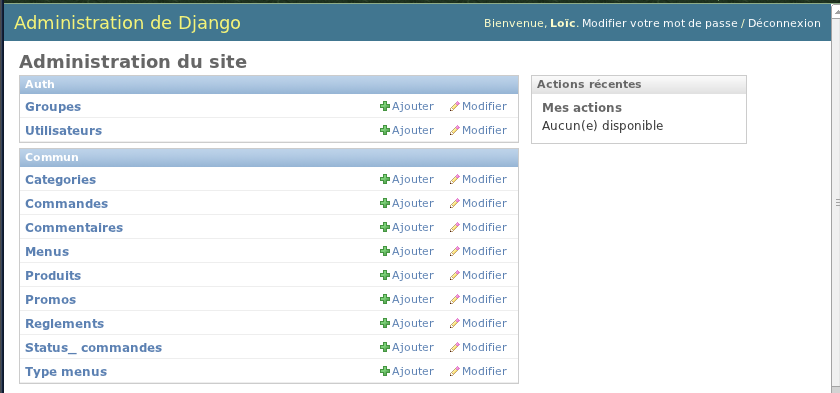
\includegraphics[width=\linewidth]{./logos/admin.png}
    \caption{L'interface d'administrationn}
\end{figure}

%%%%%%%%%%%%%%%%%%%%%%%%%%%%%%%%%%%%%%%%%%%%%%%%%%%%%%%%%%%%%%%%%%%%%%%%%%%%%%%%%%%%%%%%%%%%%%%%%%%%ù
%%%%%%%%%%%%%%%%%%%%%%%%%%%%%%%%%%%%%%%%%%%%%%%%%%%%%%%%%%%%%%%%%%%%%%%%%%%%%%%%%%%%%%%%%%%%%%%%%%%%ù
%%%%%%%%%%%%%%%%%%%%%%%%%%%%%%%%%%%%%%%%%%%%%%%%%%%%%%%%%%%%%%%%%%%%%%%%%%%%%%%%%%%%%%%%%%%%%%%%%%%%ù
\chapter{Module Compte}
% TODO Seb

    \paragraph{}Afin de pouvoir mettre en place ce site de gestion il nous fallait une gestion complète d'utilisateurs afin pouvoir définir les rôles de chacun. Django propose une gestion utilisateur permettant la gestion des rôles, des accès ... Nous allons donc détailler les fonctionnalités de ce module.

    \section{Modèle de base de données}

        \paragraph{}Django fournit une table utilisateur avec les attributs suivants par défaut :\\
        \begin{itemize}
            \item username : Login utilisateur ;\\
            \item first\_name : Prénom de l'utilisateur ;\\
            \item last\_name : Nom de famille de l'utilisateur ;\\
            \item email : Adresse email de l'utilisateur ; \\
            \item password : Mot de passe crypté ;\\
            \item is\_staff : Permet de définir le rôle de staff ;\\
            \item is\_superuser : Permet de définir le rôle d'administrateur ;\\
            \item last\_login : Dernière visite de l'utilisateur ;\\
            \item date\_joined : Date de création de l'utilisateur.\\
        \end{itemize}

        \paragraph{}Afin de compléter ce modèle fournis par défaut nous avons mis en place une table UserProfile. Nous avons ainsi pu ajouter les attributs permettant de connaitre la promotion, le panier, et la dette d'un utilisateur.

    \section{Création de compte}

        \paragraph{}Afin de créer la page de création de compte nous avons utilisé Django qui nous permet de créer des formulaires complet à partir d'un modèle de base de données. Django permet notamment d'implémenter un formulaire vérifiant la validité des champs.

        \paragraph{}Lors de la validation du formulaire les champs sont vérifiés afin de tenir compte de plusieurs contraintes. Le nom d'utilisateur ne doit pas déjà être présent dans la base de données, de même pour l'adresse email. Les deux champs mot de passe doivent de plus correspondre. Si ces contraintes sont vérifiées une entrée dans la base de données est créé pour cet utilisateur.

    \section{Identification et gestion de comptes}

        \paragraph{}Un utilisateur, une fois inscrit, peut s'identifier sur le site. L'identification est conservée sous la forme d'une session et cette identification est vérifiée pour afficher les pages autorisées pour cet utilisateur.

        \paragraph{}L'utilisateur a de plus une age gestion de comptes lui fournissant les informations stockées le concernant. Cette page contient notamment le montant de sa dette actuelle et l'historique de ses commandes, quelles que soit leurs statut.

    \section{Travail restant}
        
        \paragraph{}Il nous reste à mettre en place une fonction permettant de rappeler son mot de passe à un utilisateur lors de l'oubli de celui-ci. Il faudrait de plus que l'utilisateur puisse modifier ses informations.

        \paragraph{}Il faudrait de plus réaliser une partie administration des comptes permettant de désactiver, supprimer des comptes et d'élever ou réduire les droits d'un utilisateur.

%%%%%%%%%%%%%%%%%%%%%%%%%%%%%%%%%%%%%%%%%%%%%%%%%%%%%%%%%%%%%%%%%%%%%%%%%%%%%%%%%%%%%%%%%%%%%%%%%%%%ù
%%%%%%%%%%%%%%%%%%%%%%%%%%%%%%%%%%%%%%%%%%%%%%%%%%%%%%%%%%%%%%%%%%%%%%%%%%%%%%%%%%%%%%%%%%%%%%%%%%%%ù
%%%%%%%%%%%%%%%%%%%%%%%%%%%%%%%%%%%%%%%%%%%%%%%%%%%%%%%%%%%%%%%%%%%%%%%%%%%%%%%%%%%%%%%%%%%%%%%%%%%%ù
\chapter{Module Commandes}
% TODO Seb

%%%%%%%%%%%%%%%%%%%%%%%%%%%%%%%%%%%%%%%%%%%%%%%%%%%%%%%%%%%%%%%%%%%%%%%%%%%%%%%%%%%%%%%%%%%%%%%%%%%%ù
%%%%%%%%%%%%%%%%%%%%%%%%%%%%%%%%%%%%%%%%%%%%%%%%%%%%%%%%%%%%%%%%%%%%%%%%%%%%%%%%%%%%%%%%%%%%%%%%%%%%ù
%%%%%%%%%%%%%%%%%%%%%%%%%%%%%%%%%%%%%%%%%%%%%%%%%%%%%%%%%%%%%%%%%%%%%%%%%%%%%%%%%%%%%%%%%%%%%%%%%%%%ù
\chapter{Module Gestion Stocks}
% TODO Loïc

Le module de gestions des stocks, comme son nom l'indique, permet de gérer les stocks de la Kfet. Ce module a été en grande partie développer au cours des TP de la matière "Technologie Web Avancée".

En plus de gérer les stocks de tous les produits, c'est dans ce module que l'on peut :
\begin{itemize}
    \item Créer/modifier/supprimer des fournisseurs ;
    \item Attacher des produits à un fournisseur (création/modification/suppression) ;
    \item Réapprovisionner les produits.
\end{itemize}

Comme on peut le deviner, nous avons choisi d'attacher un produit à un fournisseur. Donc un fournisseur possède 0 ou plusieurs produits, c'est une façon de bien différencier les produits et aussi de pourvoir dans le futur enregistrer les commandes que l'on effectue au sein même de notre application web.

Pour l'instant, notre gestion de stock permet de réapprovisionner les stocks mais n'enregistre pas les commandes fournisseurs que l'on peut faire. Cette fonctionnalité sera développé dans le futur.

\section{Fonction du module}
    \subsection{Modèle de base de données}
\paragraph{Un fournisseur}
\begin{itemize}
    \item Nom ;
    \item Adresse ;
    \item Téléphone ;
    \item Mail ;
    \item Description ;
\end{itemize}

\paragraph{Un produit}
\begin{itemize}
        \item nom ;
        \item prix ;
        \item articleDouble ;
        \item info ;
        \item ingredients ;
        \item categorie : Chaque produit appartient à une catégorie (Pizza, Sandwich, Boisson, \ldots);
        \item image : Chaque produit possède son image afin d'être visible sur le site ;
        \item quantite : Quantité en stock;
        \item quantiteCommandeFournisseur : Quantité actuellement en commande ;
        \item fournisseur.
\end{itemize}

    \subsection{Fonctions du contrôleur}
\paragraph{index} Cette fonction retourne la page d'accueil du module. Elle permet de visualiser immédiatement les produits qui sont actuellement en rupture ainsi que tous les produits que peut proposer le site. Une pagination est effectuée, bien entendu, car il ne serait pas très pratique d'afficher tous les objets sur une même page. La pagination permet de n'afficher que 10 produits à la fois.

\paragraph{Creer/Modifier/Supprimer Fournisseur}

\paragraph{Creer/Modifier/Supprimer Produit}

\paragraph{Commander} Cette fonction permet de commander une certaine quantité d'un produit à son attribut quantiteCommandeFournisseur. 

%%%%%%%%%%%%%%%%%%%%%%%%%%%%%%%%%%%%%%%%%%%%%%%%%%%%%%%%%%%%%%%%%%%%%%%%%%%%%%%%%%%%%%%%%%%%%%%%%%%%ù
%%%%%%%%%%%%%%%%%%%%%%%%%%%%%%%%%%%%%%%%%%%%%%%%%%%%%%%%%%%%%%%%%%%%%%%%%%%%%%%%%%%%%%%%%%%%%%%%%%%%ù
%%%%%%%%%%%%%%%%%%%%%%%%%%%%%%%%%%%%%%%%%%%%%%%%%%%%%%%%%%%%%%%%%%%%%%%%%%%%%%%%%%%%%%%%%%%%%%%%%%%%ù
\chapter{Module Ventes}%{{{
% TODO Seb

    \paragraph{}Nous allons vous présenter dans cette partie le module de ventes du site web. Voici tout d'abord une capture d'écran de la page de ventes vue par un kftier.
    \begin{center}
        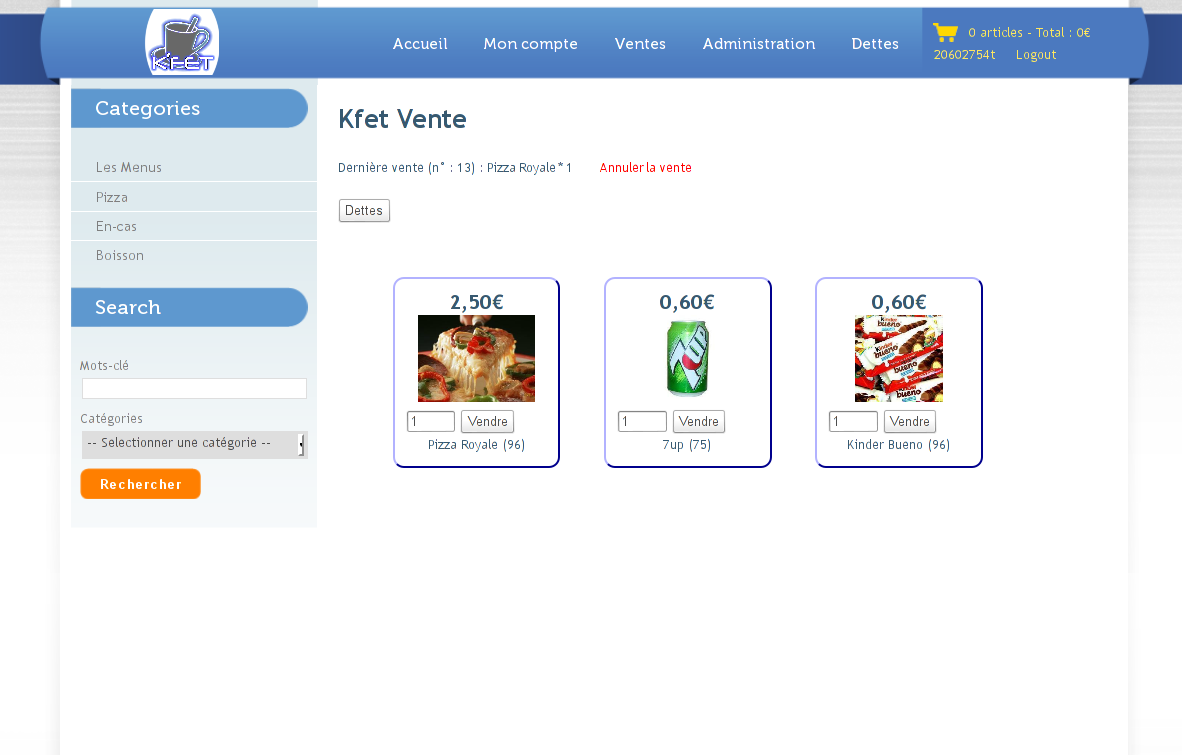
\includegraphics[width=1\linewidth]{logos/ventes.png}
    \end{center}
    \paragraph{}Nous allons dans un premier temps définir les fonctionnalités disponible dans la page, puis nous détaillerons le fonctionnement de celles-ci.

    \section{Détail des fonctionnalités}

        \paragraph{}Lorsque un kftier veut vendre un produit il se rend sur cette page. La page indique plusieurs informations : \\
            \begin{itemize}
                \item Les produits avec pour chaque produit : son prix, sa quantité restante entre parenthèse, une image le représentant ;\\
                \item Une indication "épuisé" lorsqu'un produit n'est plus disponible ;\\
                \item La dernière vente effectuée et la possibilité d'annuler celle-ci en cas d'erreur ;\\
                \item Une liste, pouvant être dissimuler, permettant de sélectionner la personne voulant payer en dette.\\
            \end{itemize}

    \section{Fonctionnement du module}

        \subsection{Modèle de base de donnée}

            \paragraph{}Les attributs de la table vente, permettant de stocker les informations de vente sont les suivants :\\
            \begin{itemize}
                \item produit\_id : identifiant du produit venu ;\\
                \item date : la date de la vente ;\\
                \item quantite : la quantité vendue ;\\
                \item user\_id : identifiant de l'utilisateur en cas de vente avec dette.
            \end{itemize}

        \subsection{Fonction du contrôleur}

            \paragraph{index}Cette fonction permet d'afficher l'index des ventes. Elle récupère tous les produits à afficher et vérifie leurs disponibilités. Elle récupère de plus la dernière vente effectuée.

            \paragraph{produit\_vente}Cette fonction permet de réaliser une vente. Elle vérifie la présence ou non de la sélection d'une personne et effectue la vente. Dans le cas où une personne est sélectionnée elle augmente la dette de celle-ci du montant de la vente. Les stocks sont de plus déduit en fonction de la quantité sélectionnée.
            \paragraph{annuler\_vente}Cette fonction annule la dernière vente effectuée en supprimant l'entrée de la base de donnée. Le stock est réapprovisionner et si une dette a été ajoutée elle est annulée.

        \subsection{Fonction du template}

            \paragraph{}Le template réalisant l'affichage de la page est formée de plusieurs formulaires et ayant chacun leurs boutons de validation.

            \paragraph{}Du javascript a été nécessaire pour la sélection du nom de la personne à ajouter en dette, en effet une seule sélection est répercutée sur tous les formulaires de la page.

            \paragraph{}Enfin une pagination est mise en place à l'aide de Django et définie à la fois dans le contrôleur et la vue.%}}}

%%%%%%%%%%%%%%%%%%%%%%%%%%%%%%%%%%%%%%%%%%%%%%%%%%%%%%%%%%%%%%%%%%%%%%%%%%%%%%%%%%%%%%%%%%%%%%%%%%%%ù
%%%%%%%%%%%%%%%%%%%%%%%%%%%%%%%%%%%%%%%%%%%%%%%%%%%%%%%%%%%%%%%%%%%%%%%%%%%%%%%%%%%%%%%%%%%%%%%%%%%%ù
%%%%%%%%%%%%%%%%%%%%%%%%%%%%%%%%%%%%%%%%%%%%%%%%%%%%%%%%%%%%%%%%%%%%%%%%%%%%%%%%%%%%%%%%%%%%%%%%%%%%ù
\chapter{Module Administration}
% TODO Loic

%%%%%%%%%%%%%%%%%%%%%%%%%%%%%%%%%%%%%%%%%%%%%%%%%%%%%%%%%%%%%%%%%%%%%%%%%%%%%%%%%%%%%%%%%%%%%%%%%%%%ù
%%%%%%%%%%%%%%%%%%%%%%%%%%%%%%%%%%%%%%%%%%%%%%%%%%%%%%%%%%%%%%%%%%%%%%%%%%%%%%%%%%%%%%%%%%%%%%%%%%%%ù
%%%%%%%%%%%%%%%%%%%%%%%%%%%%%%%%%%%%%%%%%%%%%%%%%%%%%%%%%%%%%%%%%%%%%%%%%%%%%%%%%%%%%%%%%%%%%%%%%%%%ù
\chapter{Module dettes}
% TODO Loïc

%%%%%%%%%%%%%%%%%%%%%%%%%%%%%%%%%%%%%%%%%%%%%%%%%%%%%%%%%%%%%%%%%%%%%%%%%%%%%%%%%%%%%%%%%%%%%%%%%%%%ù
%%%%%%%%%%%%%%%%%%%%%%%%%%%%%%%%%%%%%%%%%%%%%%%%%%%%%%%%%%%%%%%%%%%%%%%%%%%%%%%%%%%%%%%%%%%%%%%%%%%%ù
%%%%%%%%%%%%%%%%%%%%%%%%%%%%%%%%%%%%%%%%%%%%%%%%%%%%%%%%%%%%%%%%%%%%%%%%%%%%%%%%%%%%%%%%%%%%%%%%%%%%ù
\chapter{Conclusion}
% TODO Loïc

%%%%%%%%%%%%%%%%%%%%%%%%%%%%%%%%%%%%%%%%%%%%%%%%%%%%%%%%%%%%%%%%%%%%%%%%%%%%%%%%%%%%%%%%%%%%%%%%%%%%ù
%%%%%%%%%%%%%%%%%%%%%%%%%%%%%%%%%%%%%%%%%%%%%%%%%%%%%%%%%%%%%%%%%%%%%%%%%%%%%%%%%%%%%%%%%%%%%%%%%%%%ù
%%%%%%%%%%%%%%%%%%%%%%%%%%%%%%%%%%%%%%%%%%%%%%%%%%%%%%%%%%%%%%%%%%%%%%%%%%%%%%%%%%%%%%%%%%%%%%%%%%%%ù
%%%%%%%%%%%%%%%%%%%%%%%%%%%%%%%%%%%%%%%%%%%%%%%%%%%%%%%%%%%%%%%%%%%%%%%%%%%%%%%%%%%%%%%%%%%%%%%%%%%%ù
%%%%%%%%%%%%%%%%%%%%%%%%%%%%%%%%%%%%%%%%%%%%%%%%%%%%%%%%%%%%%%%%%%%%%%%%%%%%%%%%%%%%%%%%%%%%%%%%%%%%ù

\end{document}

